% Conceptual Framework for: Bayesian Causal Inference on AI Grading Effects on Student Performance

\section{Conceptual Framework}

To estimate the causal effects of automated assessment, we developed a Directed Acyclic Graph (DAG) grounded in established theoretical frameworks. We draw on Algorithm Aversion theory \citep{dietvorst2015algorithm} and Self-Regulated Learning \citep{zimmerman2000attaining}. Figure \ref{fig:dag} maps the hypothesized causal pathways and identification assumptions.

\begin{figure}[ht]
    \centering
    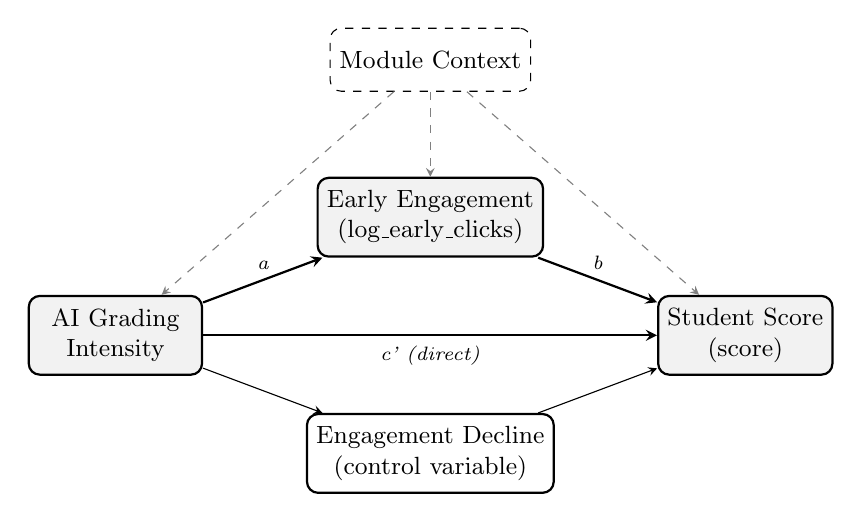
\begin{tikzpicture}[
        node distance=2.5cm,
        main/.style={draw, rounded corners, minimum width=2.2cm, minimum height=1cm, align=center, font=\small, fill=gray!10, thick},
        control/.style={draw, rounded corners, minimum width=2.2cm, minimum height=1cm, align=center, font=\small, fill=white, thick},
        conf/.style={draw, rectangle, rounded corners, minimum width=2cm, minimum height=0.8cm, align=center, font=\small, dashed, fill=white},
        arrow/.style={->, thick, >=stealth},
        dasharrow/.style={->, dashed, >=stealth, gray},
        label/.style={font=\scriptsize\itshape}
    ]
        \node[main] (AI) at (0, 0) {AI Grading\\Intensity};
        \node[main] (Early) at (4, 1.5) {Early Engagement\\(log\_early\_clicks)};
        \node[control] (Traj) at (4, -1.5) {Engagement Decline\\(control variable)};
        \node[main] (Score) at (8, 0) {Student Score\\(score)};
        \node[conf] (Conf) at (4, 3.5) {Module Context};
        \draw[arrow] (AI) -- (Early) node[label, midway, above] {a};
        \draw[arrow] (Early) -- (Score) node[label, midway, above] {b};
        \draw[arrow] (AI) -- (Score) node[label, midway, below] {c' (direct)};
        \draw[arrow, thin] (AI) -- (Traj);
        \draw[arrow, thin] (Traj) -- (Score);
        \draw[dasharrow] (Conf) -- (AI);
        \draw[dasharrow] (Conf) -- (Early);
        \draw[dasharrow] (Conf) -- (Score);
    \end{tikzpicture}
    \caption{Causal DAG. Paths a and b represent formal mediation through Early Engagement. Path c' is the direct effect. Engagement Decline is a control variable. Module Context is a confounder controlled via hierarchical random effects.}
    \label{fig:dag}
\end{figure}

\subsection{Theoretical Assumptions and Causal Pathways}

The DAG posits three structural mechanisms linking AI grading intensity to student outcomes. The first pathway (path a) captures the effect of AI grading on student engagement. We hypothesize that exposure to automated assessment influences how students interact with the learning platform. Behavioral research suggests that algorithm aversion may reduce student effort when they perceive automated systems as untrustworthy \citep{dietvorst2015algorithm}. Conversely, rapid automated feedback might reinforce engagement through the feedback loops described in self-regulated learning theory \citep{saqr2025engagement}.

The second pathway (path b) represents the effect of engagement on academic performance. We assume that engagement causally drives student scores. This relationship is well-established in the learning analytics literature, where behavioral engagement proxies the cognitive effort required for mastery \citep{zhang2023learning}.

The third mechanism is the direct effect of AI grading on scores (path c'), which captures pathways unrelated to engagement. If AI systems grade systematically differently from humans due to algorithmic characteristics, this will manifest as a direct effect on scores \citep{huang2025ai}. Student effort does not mediate this pathway.

\subsection{Identification Strategy}

A critical threat to causal identification is unmeasured institutional confounding. Easy modules might employ more AI grading and yield higher scores, creating a spurious positive association. Certain course designs might encourage both high automation and high engagement. Such confounds would bias naive estimates.

We address this via the backdoor criterion by conditioning on Module Context through hierarchical random intercepts. This approach blocks non-causal paths by absorbing module-level heterogeneity. The identifying assumption is that within a given module presentation, variation in AI grading intensity is effectively random after conditioning on the hierarchical structure.
